\documentclass[11pt,a4paper]{article}
\usepackage{fontspec}
\setmainfont{TeX Gyre Pagella}
\newfontfamily\headfont{Inter}[UprightFont=*-ExtraBold,BoldFont=*-ExtraBold,Extension=.otf,Path=/usr/share/fonts/opentype/inter/]
\usepackage[a4paper,margin=2.3cm]{geometry}
\usepackage{graphicx,booktabs,float,caption,array,xcolor,longtable}
\usepackage{xurl}
\usepackage[hidelinks]{hyperref}
\usepackage{titlesec}
\usepackage[round]{natbib}
\usepackage{setspace}
\setstretch{1.05}
\renewcommand{\topfraction}{0.9}
\renewcommand{\bottomfraction}{0.8}
\renewcommand{\textfraction}{0.1}
\renewcommand{\floatpagefraction}{0.75}
\setlength{\parindent}{0pt}
\setlength{\parskip}{0.55em}
\titleformat{\section}{\headfont\Large}{\thesection}{0.8em}{}
\titleformat{\subsection}{\headfont\large}{\thesubsection}{0.8em}{}
\captionsetup{font=small,labelfont=bf}
\urlstyle{same}
\hypersetup{pdftitle={How Close Did Ino Get?},pdfauthor={Tristan Hotham}}

\begin{document}
\begin{center}
{\Large\bfseries How Close Did Ino Get?\par}
\vspace{0.4em}
{\large Measuring 28 sheets of Ino Tadataka's large-scale map of Japan (1821)\\against the modern coastline\par}
\vspace{1.2em}
{\large Tristan Hotham\par}
\vspace{0.3em}
{\small Independent researcher\\
ORCID: 0000-0003-4931-9349\\
DOI: https://doi.org/10.5281/zenodo.23882609\par}
\vspace{0.8em}
2026
\end{center}

\begin{quote}
\small
\begin{center}\textbf{Abstract}\end{center}
Ino Tadataka's survey map of Japan, completed in 1821, is celebrated for its accuracy. I test that reputation on the 40 sheets of the large-scale set (Dai Nihon Enkai Yochi Zenzu) held in manuscript copy by the Library of Congress and photographed on Wikimedia Commons, which cover Hokkaido, the southern Kurils and part of Sakhalin at a nominal 1:43,600. Each sheet was placed by matching its drawn coastline to Natural Earth's 1:10m coast, and 28 were located. Allowing each sheet only one shift and one rotation at the nominal scale, the drawn coast of a typical sheet lies a median 280 m from the modern coast (6.4 mm on the paper), with 90\% within 1 km; 1,494 km of drawn coast were measured. 93 control points (23 picked by eye, 70 matched automatically) lie a median 543 m from their true positions. Sheets whose coast fixes the angle are rotated a median 1.3 degrees from true north, and the best-fitting scales of well-controlled sheets agree within 5\%; neither affine nor quadratic fits improve on a similarity transform. On the 1878 Army General Staff map of the whole country, compiled from Ino's survey, 18 capes and islands lie a median 7.9 km from a best-fitting modern position, with north-south and east-west errors of similar size and a marginal east-west stretch of 1.9\%. All figures are upper bounds on survey error, since they include copying, paper distortion and the generalisation of the modern coastline.

\textbf{Keywords:} Ino Tadataka; historical cartography; map accuracy; georeferencing; Hokkaido; Edo period; open data
\end{quote}

\section{Introduction}
Ino Tadataka (1745 to 1818) was a merchant who ran a sake brewing business in Sawara and, after retiring, studied astronomy in Edo. From 1800 he led a series of surveys that measured Japan's coasts and main roads by traverse, with distances paced or chained, bearings by compass and latitudes by star observations. The survey's maps were completed by his team in 1821, after his death in 1818, as the Dai Nihon Enkai Yochi Zenzu: 214 large-scale sheets at 1:36,000, with Hokkaido and part of northern Japan at 1:43,600, and medium and small-scale versions. The map is widely described as remarkably accurate. This study asks how accurate, for the part of the large-scale set that is openly available as photographs: how far its drawn coast lies from the modern coast, how far identifiable features are displaced, whether the sheets are rotated or out of scale, and, at the national scale, whether latitude and longitude errors differ. The paper accompanies an interactive comparison (\url{https://maps.tristanhotham.com/ino-japan/}).

\section{Data}
\textbf{The sheets.} The Library of Congress holds a manuscript copy of the large-scale map (Geography and Map Division, item 2001620020). Wikimedia Commons has photographs of sheets 1 to 40, used here reduced to 3,840 pixels wide (public domain). All 40 show the far north. They are drawn in ink and watercolour: land is shown by green hachures, the surveyed coast by an ink line, and the sea is left blank. Several sheets carry a pencil grid; 8 are unfinished pencil drafts of inland routes.

\textbf{The national map.} Dai Nihon Zenzu, published in 1878 by the Army General Staff Bureau and compiled from Ino's survey (Wikimedia Commons, 1,885 pixels wide, public domain).

\textbf{The modern coast.} Natural Earth's 1:10m countries for Japan and the Russian-administered islands \citep{naturalearth}. This is the only modern coastline used, and its generalisation sets a floor under every error reported here.

\section{Methods}
\subsection{Extracting the drawn coast}
On each sheet, at a quarter of the working resolution, a pixel is taken as coast if it is dark or red ink, lies within six quarter-pixels of green hachure, and belongs to an ink stroke at least 40 quarter-pixels long, which removes most labels. Masks of land and sea near the coast are kept for the placement search. The coast is thinned to one point per 8 by 8 pixel cell.

\subsection{Placing the sheets}
Each sheet was placed by brute force: for three scales around the nominal and rotations from minus 15 to plus 15 degrees in 3 degree steps, the sheet's land and sea masks were correlated with modern land and sea on a 1 km grid, by FFT. The best placements were inspected by eye on overlays; 28 were accepted, one (sheet 14) failed, and 12 sheets in all were left unplaced. Each accepted sheet was then fitted to the modern coast by trimmed iterative closest point, allowing a rotation and a translation with the scale fixed. The nominal scale in ground metres per pixel of the full-size photograph was calibrated on sheet 5, whose hooked Notsuke spit fixes it (6.66 m per pixel, about 166 pixels per inch at 1:43,600), and carried to the other sheets through each photograph's known pixel size. All measurements are on a Lambert conformal conic projection with standard parallels 33 and 44 degrees; rotations are corrected for meridian convergence and so are relative to true north.

\subsection{Coastline agreement}
Along the drawn coast of each located sheet, a checkpoint was taken every kilometre (so the number of checkpoints is the length of drawn coast in km), and for every drawn coast point the distance to the nearest modern coast was measured after the fit. Each sheet is summarised by the median distance and the shares within 250 m, 500 m and 1 km.

\subsection{Control points}
A coastline constrains position across the shore but not along it. Two kinds of control point constrain both. (a) 23 capes, spit tips and bends were picked by eye on overlays of the sheet and the modern coast, where both show the same feature, with a confidence grade; their modern positions are the nearest Natural Earth coast vertex to the feature. (b) Every 3 km along the drawn coast, a window 8 km across was matched to the modern coast by a local translation (iterative closest point after the sheet's fit); a window became a control point only if the modern coast it matched turns enough to fix the shift in both directions (smaller to larger eigenvalue of the summed outer product of coast normals at least 0.10), its matched points lay within a median 600 m and the shift was under 3 km. This gave 70 points. The error of a control point is the distance between its true position and where the sheet's coastline fit puts it; the control points are not used in that fit. On sheets with at least four control points I also fitted similarity, affine (six or more points) and quadratic (twelve or more) transformations of sheet pixels to modern positions and computed leave-one-out errors.

\subsection{National check}
On the 1878 map I picked 18 features by eye: capes at the extremities of Honshu, Shikoku and Kyushu and the centres of 5 islands. They were fitted to their modern positions by a similarity transform and by an affine transform; residuals were split into north-south and east-west parts, and the ratio of east-west to north-south scale in the affine fit was bootstrapped (2,000 resamples).

\section{Results}
\subsection{Where the sheets are}
Figure~\ref{fig:overview} shows the 28 located sheets. They follow the coast round Hokkaido and out to Kunashiri, Iturup and Sakhalin: 7 on the Japan Sea coast, 8 on the Pacific coast, 6 on the Okhotsk coast, 3 around Nemuro and Kushiro, 3 in the Kurils and 1 in Sakhalin. Table~\ref{tab:sheets} lists them.

\begin{figure}[tbp]\centering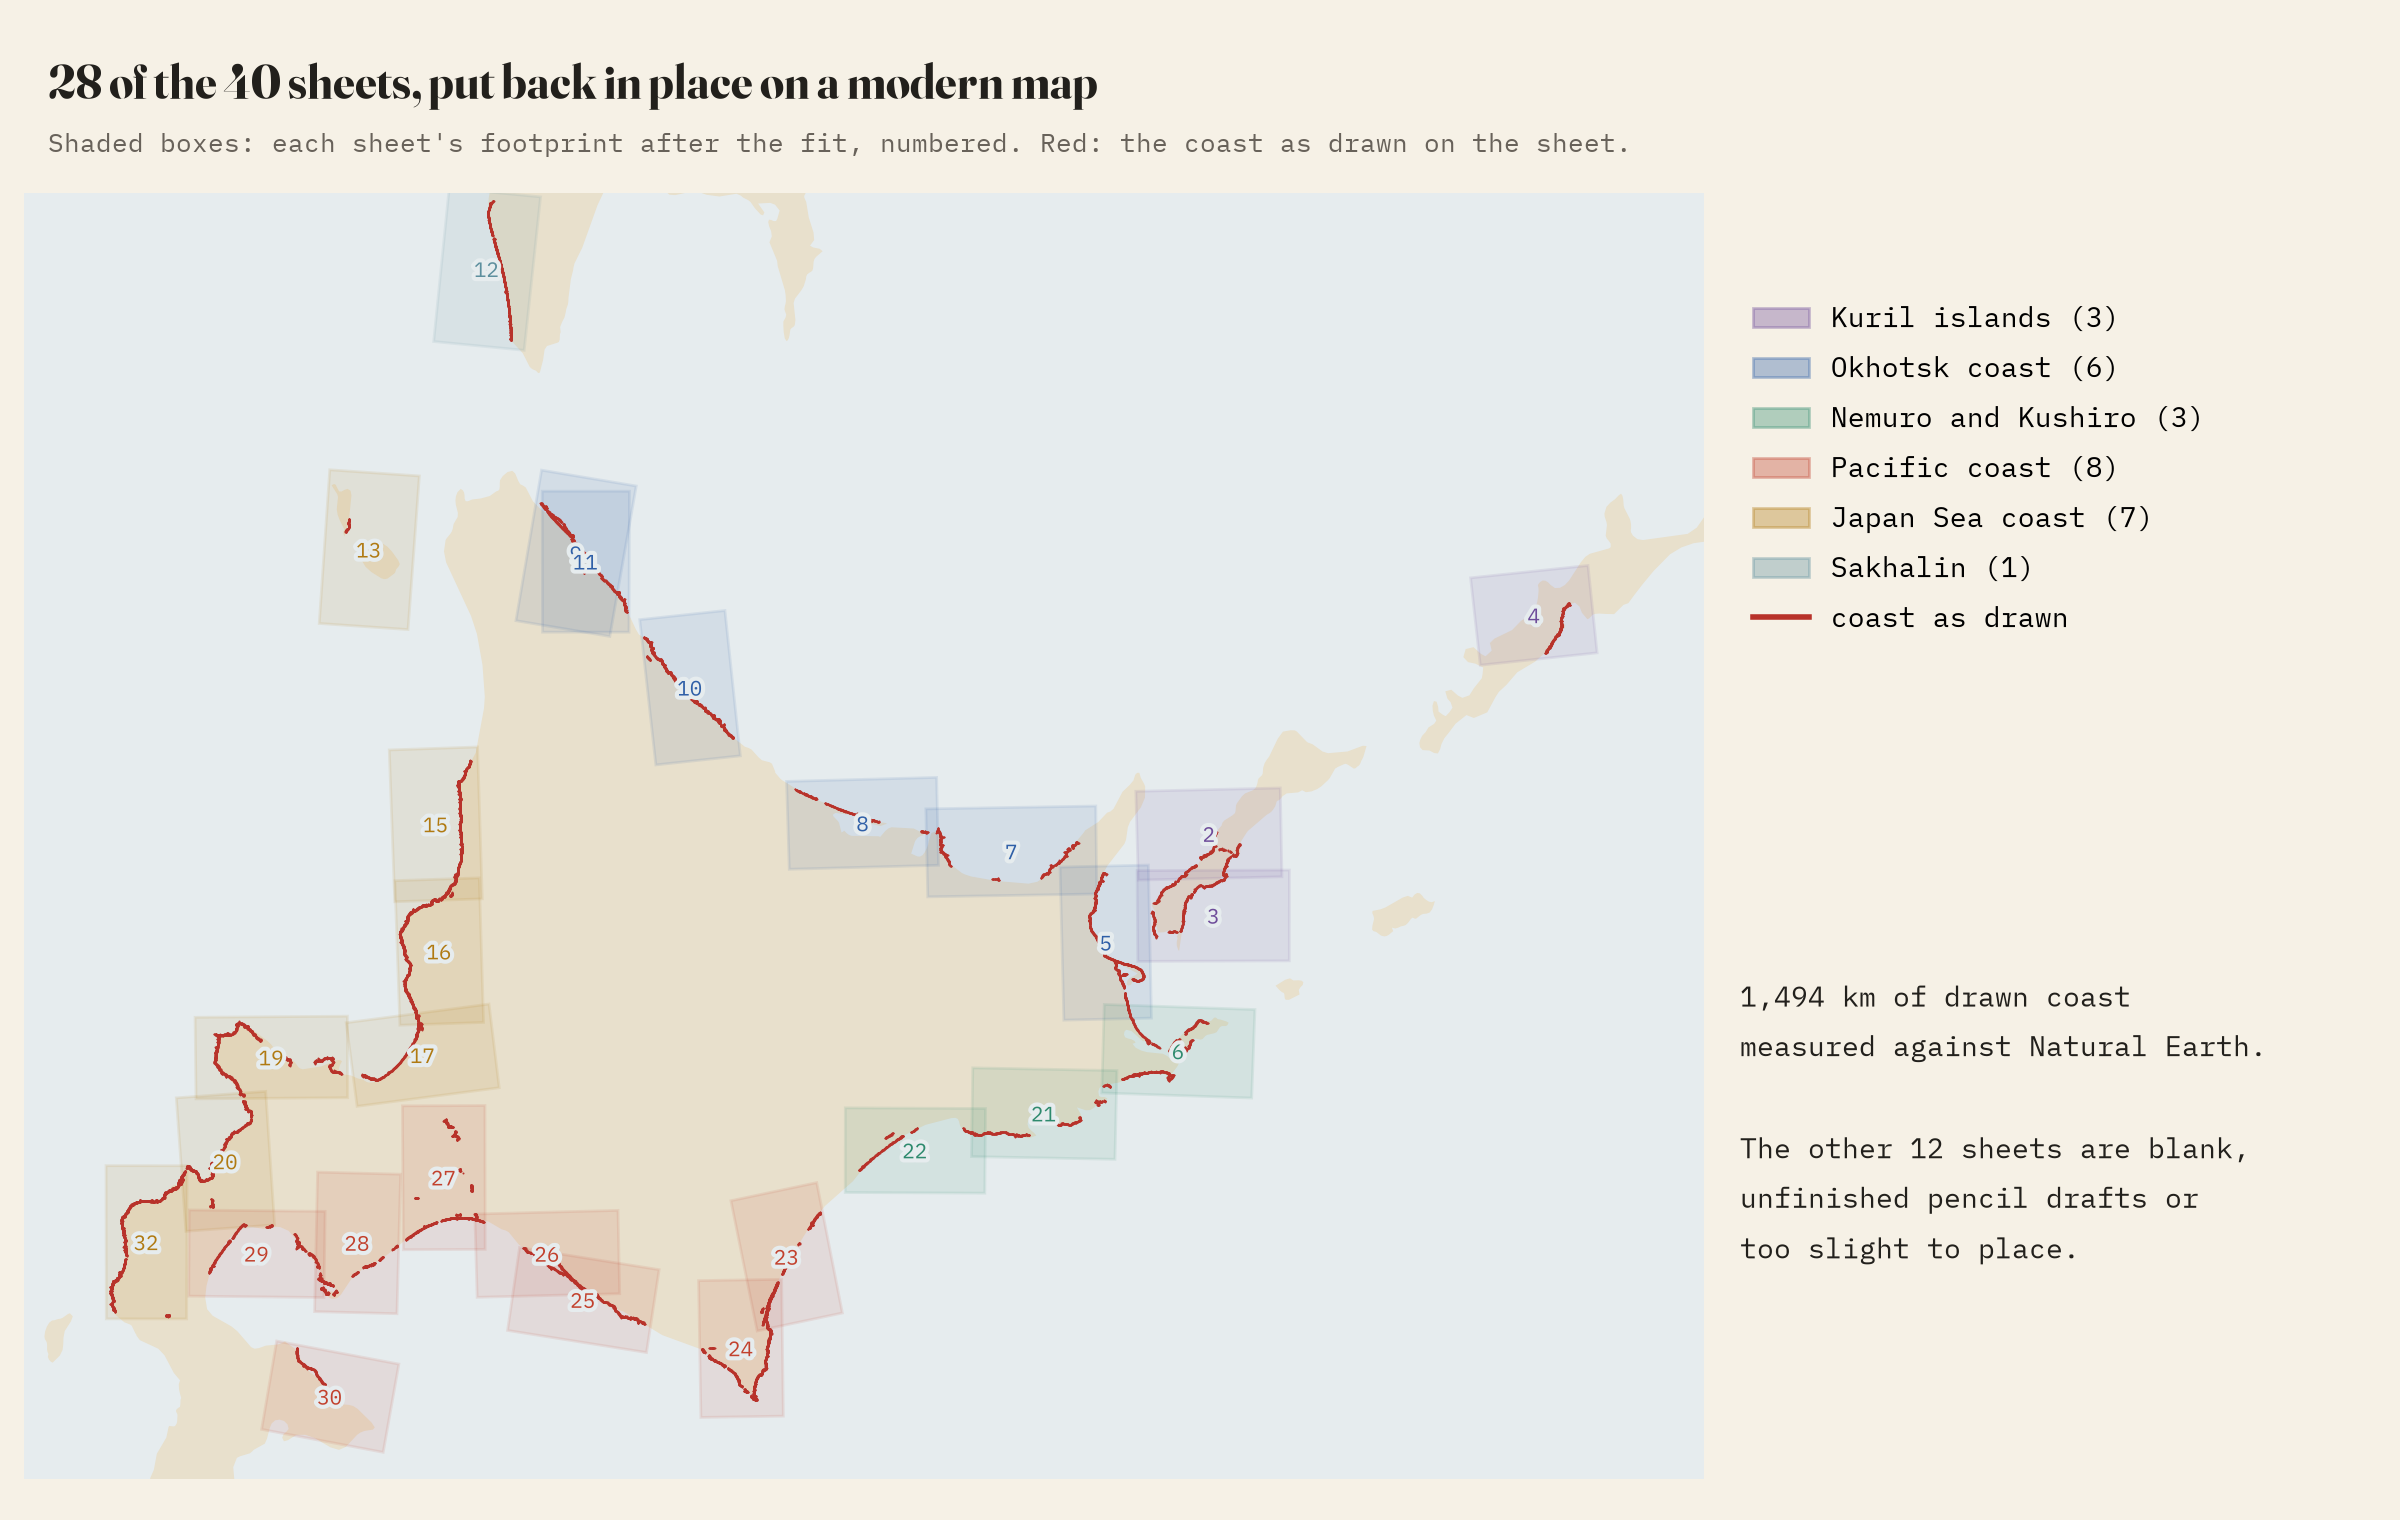
\includegraphics[width=\textwidth]{f_overview.png}
\caption{The 28 located sheets on a modern map, with the drawn coast in red.}\label{fig:overview}\end{figure}

\subsection{Coastline agreement}
After one shift and one rotation per sheet at the nominal scale, the median distance from the drawn coast to the modern coast is 280 m on a typical sheet (median over sheets), ranging from 108 m (sheet 26, Hidaka-Monbetsu) to 651 m (sheet 25, Shizunai); 15 sheets are under 300 m and 5 over 500 m (Figure~\ref{fig:coast}). On a typical sheet 45\% of the drawn coast is within 250 m, 69\% within 500 m and 90\% within 1 km (Figure~\ref{fig:spread}). At 1:43,600, the median gap is 6.4 mm on the paper, about 13 times a drafting error of 0.5 mm (22 m).

\begin{figure}[tbp]\centering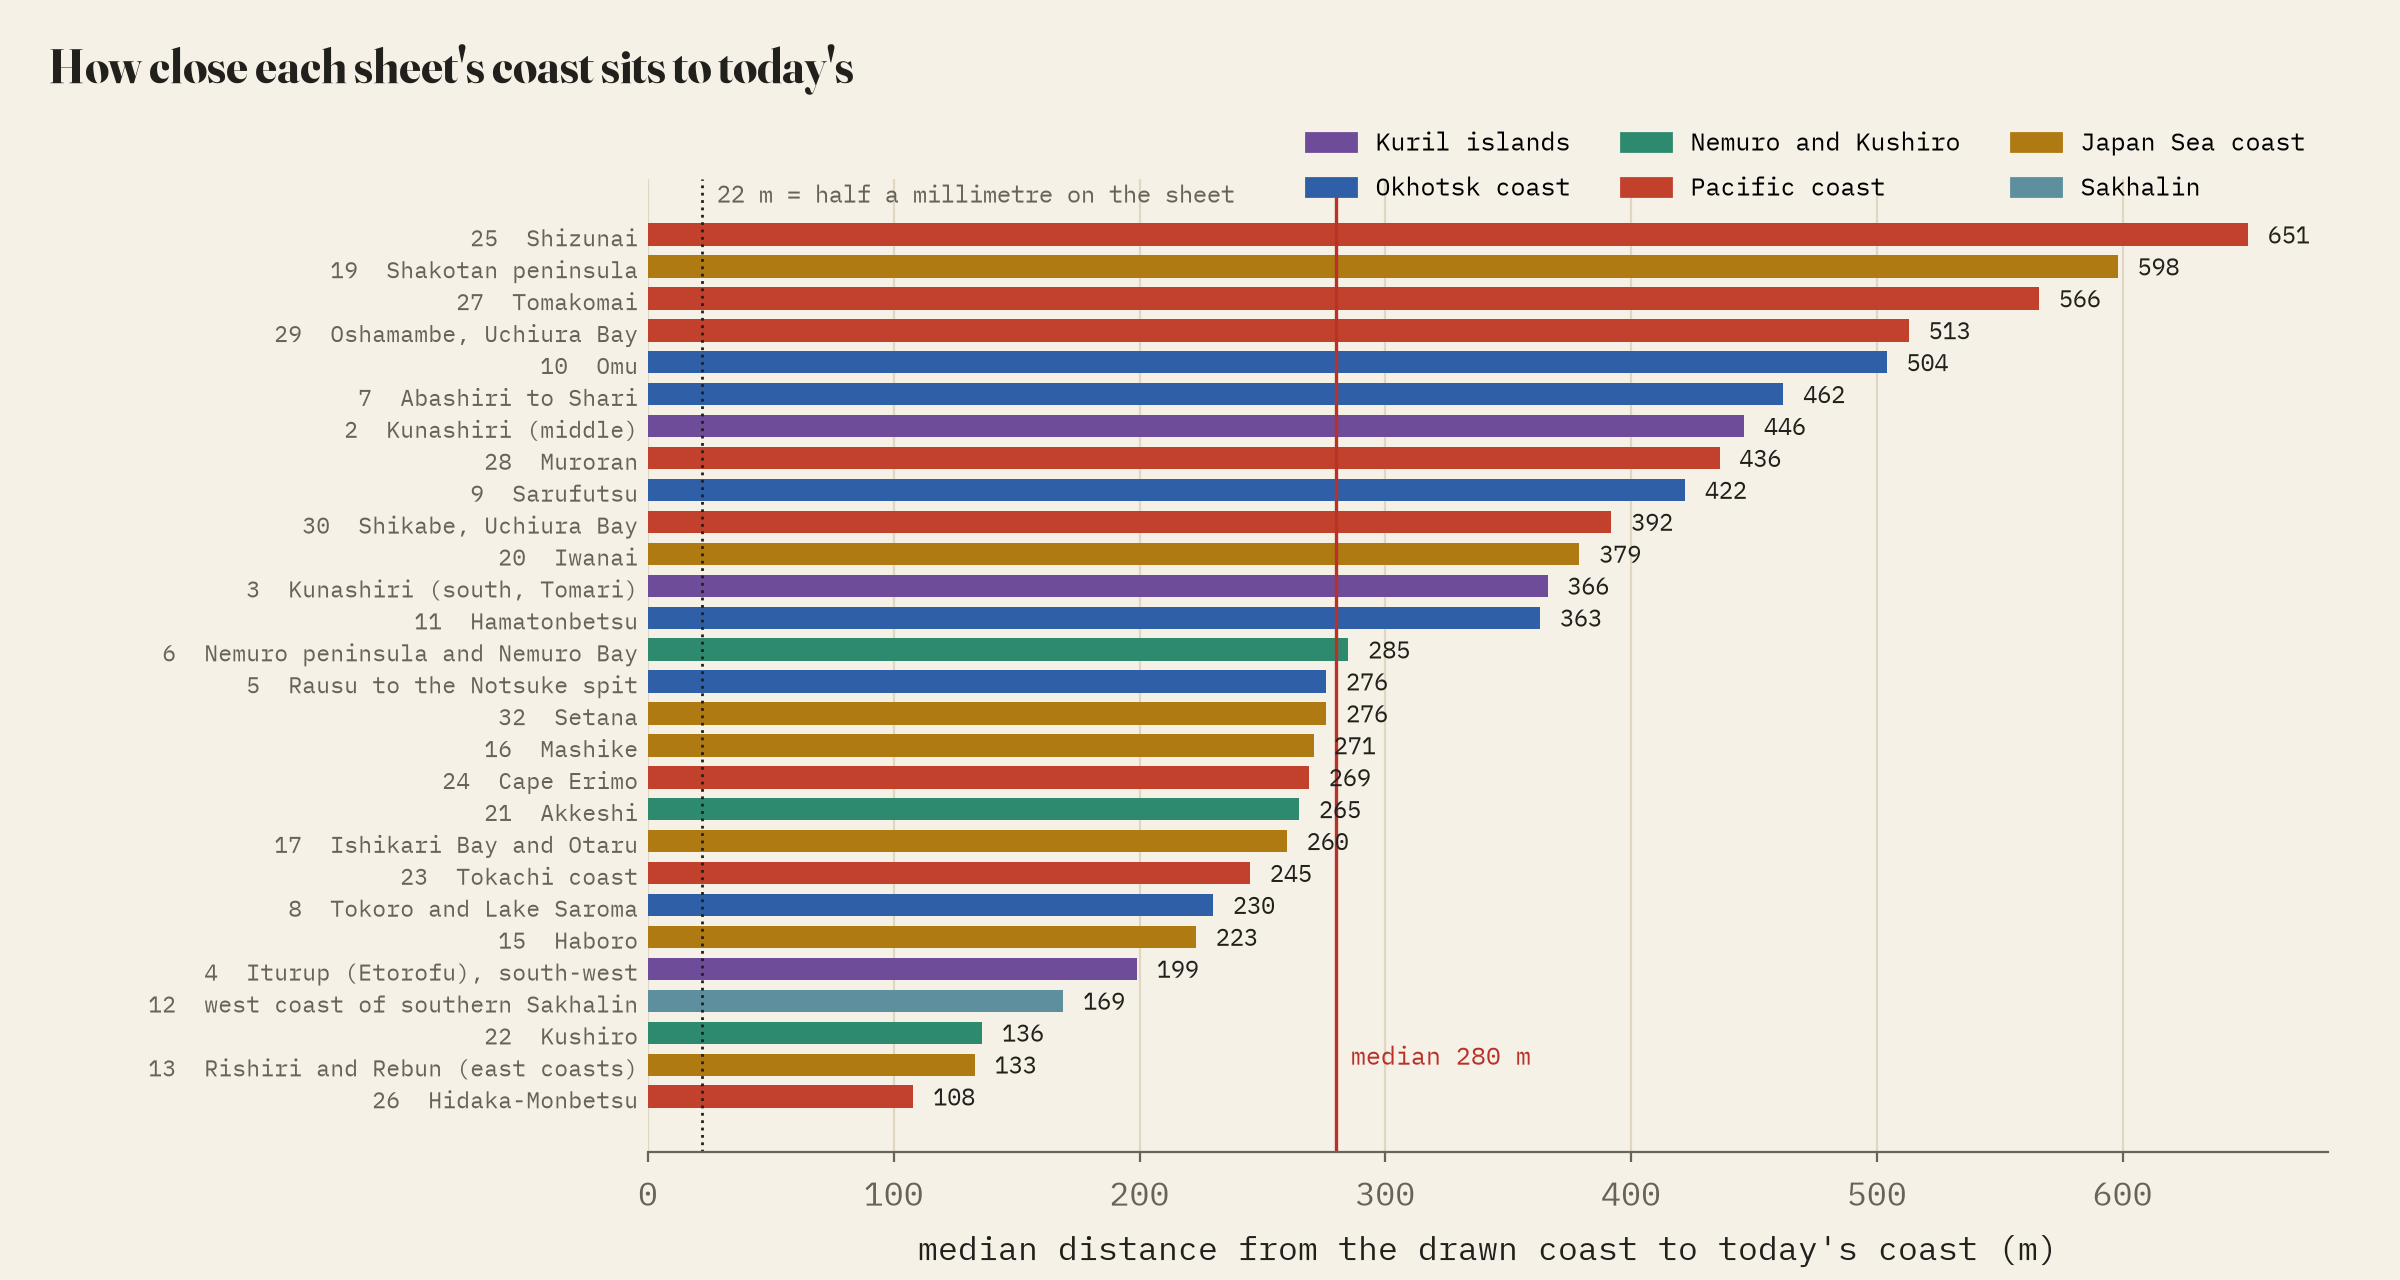
\includegraphics[width=\textwidth]{f_coast.png}
\caption{Median distance from each sheet's drawn coast to the modern coast after a rigid fit at the nominal scale.}\label{fig:coast}\end{figure}

\begin{figure}[tbp]\centering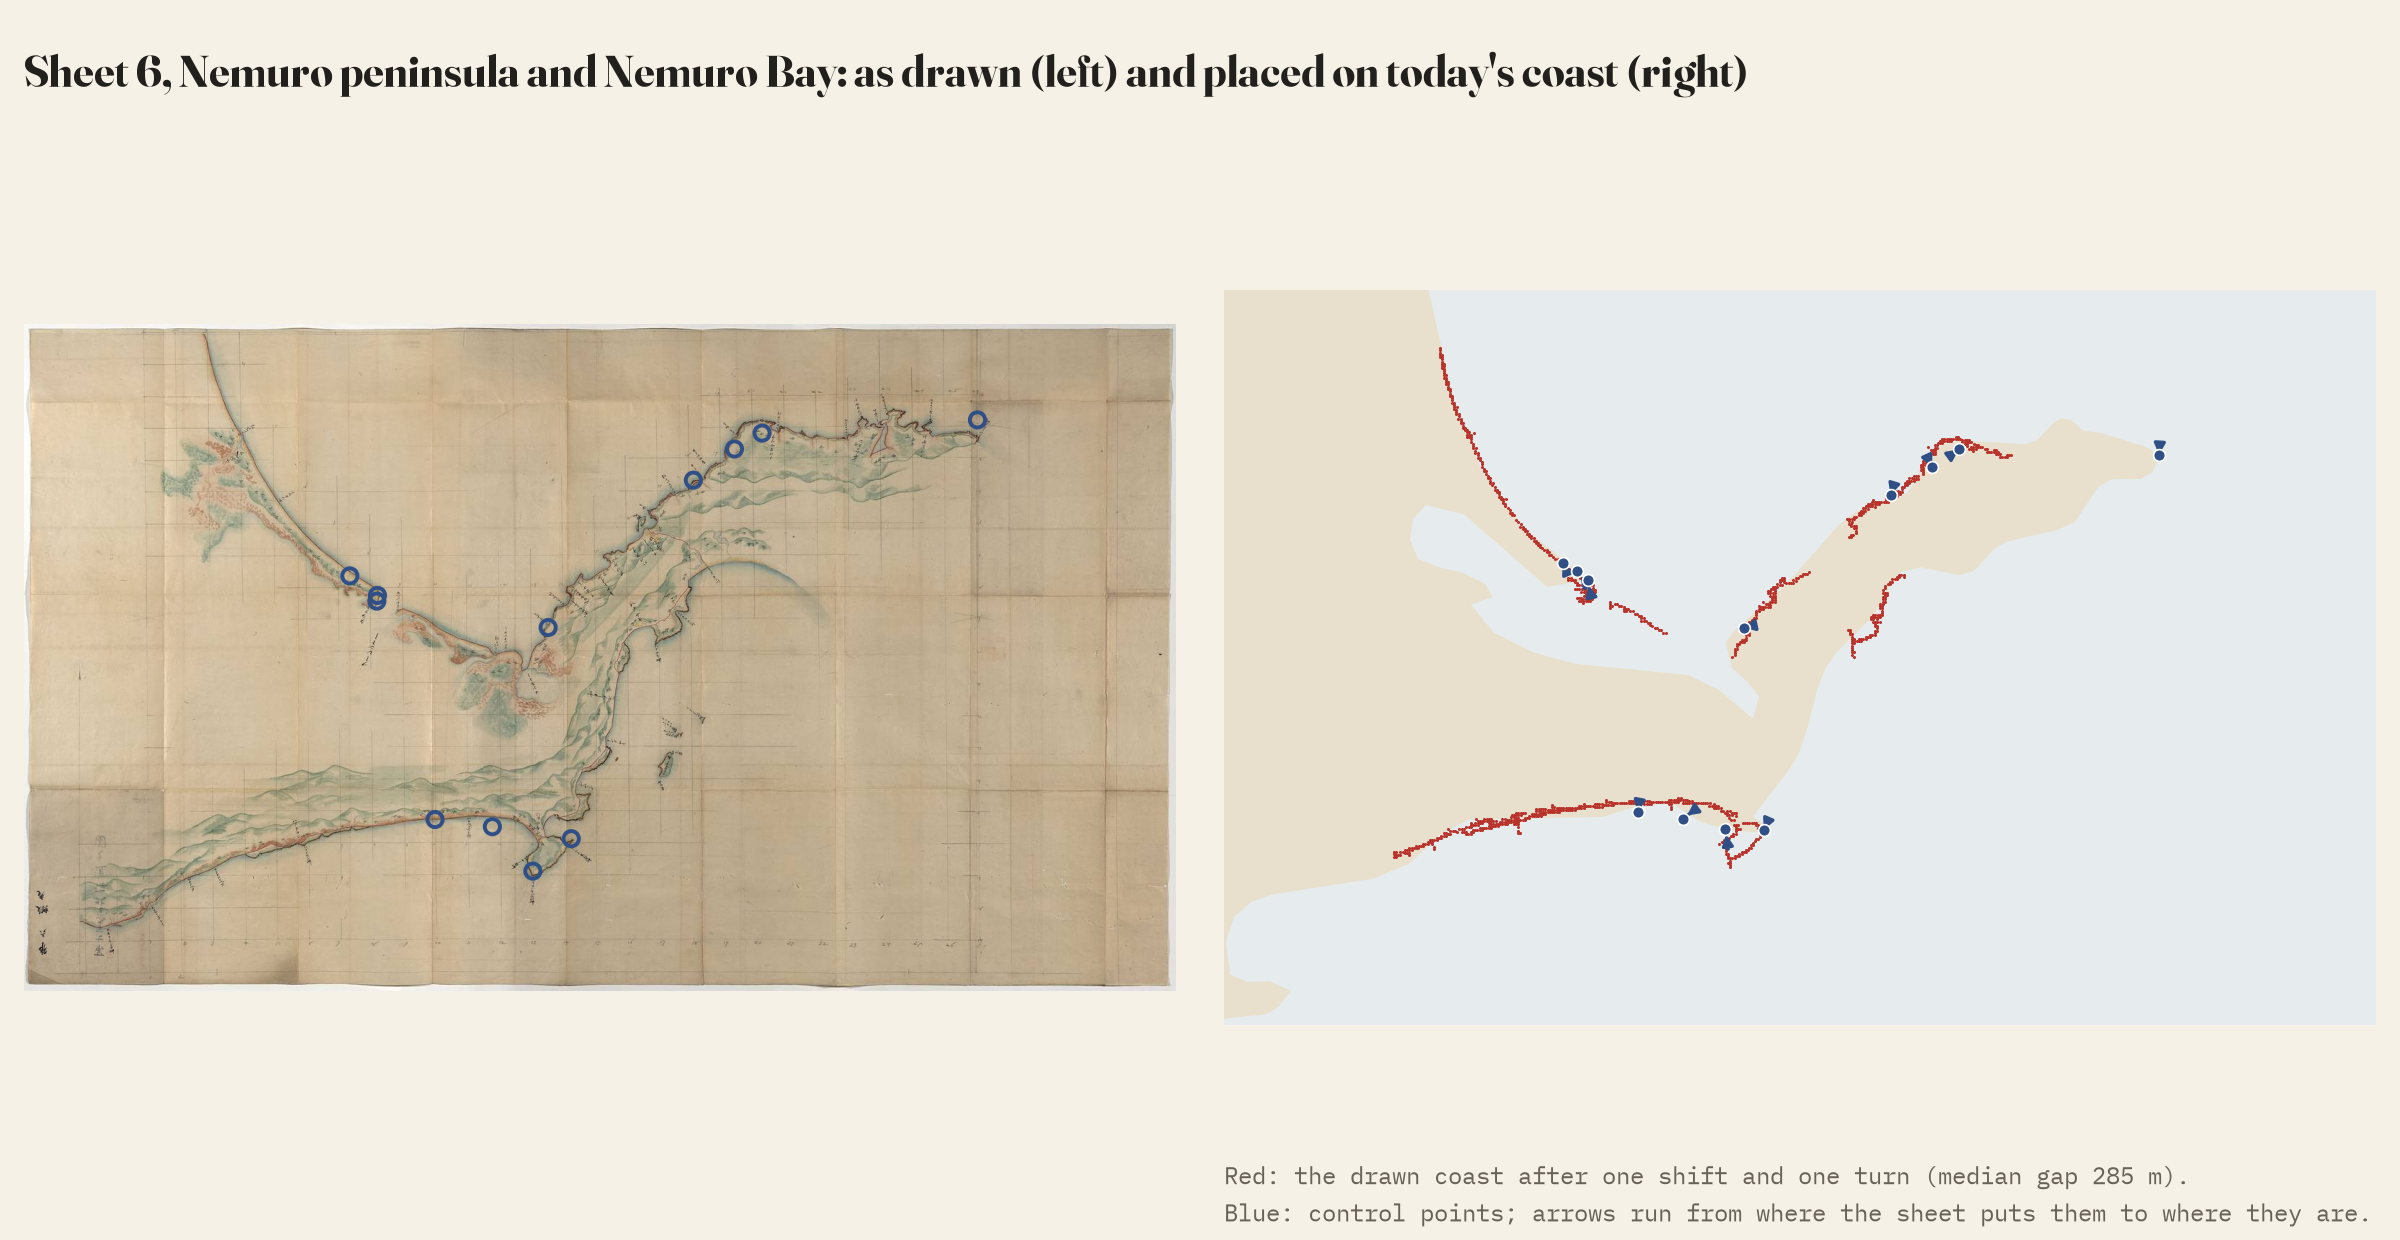
\includegraphics[width=\textwidth]{f_sheet.png}
\caption{Sheet 6 (Nemuro peninsula and Nemuro Bay) as drawn and placed on the modern coast, with its control points.}\label{fig:sheet}\end{figure}

\subsection{Control points}
I found 93 control points on 16 sheets, short of the 250 I aimed for; only 6 sheets have eight or more. Their median error is 543 m (870 m for the hand-picked points, 481 m for the automatic ones); 45\% are under 500 m and 72\% under 1 km, and the largest is 2,702 m, at Cape Erimo. Of the named capes picked with high confidence, Cape Nosappu is 585 m from its modern position, Cape Notoro 531 m and the tip of the Shakotan peninsula 557 m.

On the 10 sheets with four or more control points, a similarity transform predicts a left-out point to a median 508 m. On the 6 sheets with six or more, an affine transform gives 536 m against 536 m for the similarity; on the 2 sheets with twelve or more, a quadratic gives 824 m against 448 m for the affine. The control points therefore show no distortion within sheets beyond a shift, a rotation and a scale.

\subsection{Rotation and scale}
On the 15 sheets whose coast curves enough to fix the angle (the same eigenvalue ratio, over the whole sheet, at least 0.15), the rotation from true north has a median of 0.9 degrees and a median absolute value of 1.3 degrees, from -1.9 to 7.3; 12 are within 2 degrees. On the 6 sheets with six or more control points, the similarity scale relative to the nominal is 0.95 to 1.03 (median 0.99).

\subsection{The national map}
On the 1878 map (Figure~\ref{fig:national}), the 18 features lie a median 7.9 km from their best-fitting positions (maximum 16.1 km, Ashizuri-misaki). Root mean square errors are 6.2 km north-south and 7.1 km east-west; the median absolute errors are 2.4 minutes of latitude and 2.0 minutes of longitude. Neither component trends with longitude (slopes 0.39 and -0.22 km per degree). In the affine fit east-west distances are 1.9\% longer than north-south ones (95\% bootstrap interval 0.1 to 3.8\%). With a map scale of 0.75 km per pixel, three pixels of picking uncertainty is 2.3 km.

\begin{figure}[tbp]\centering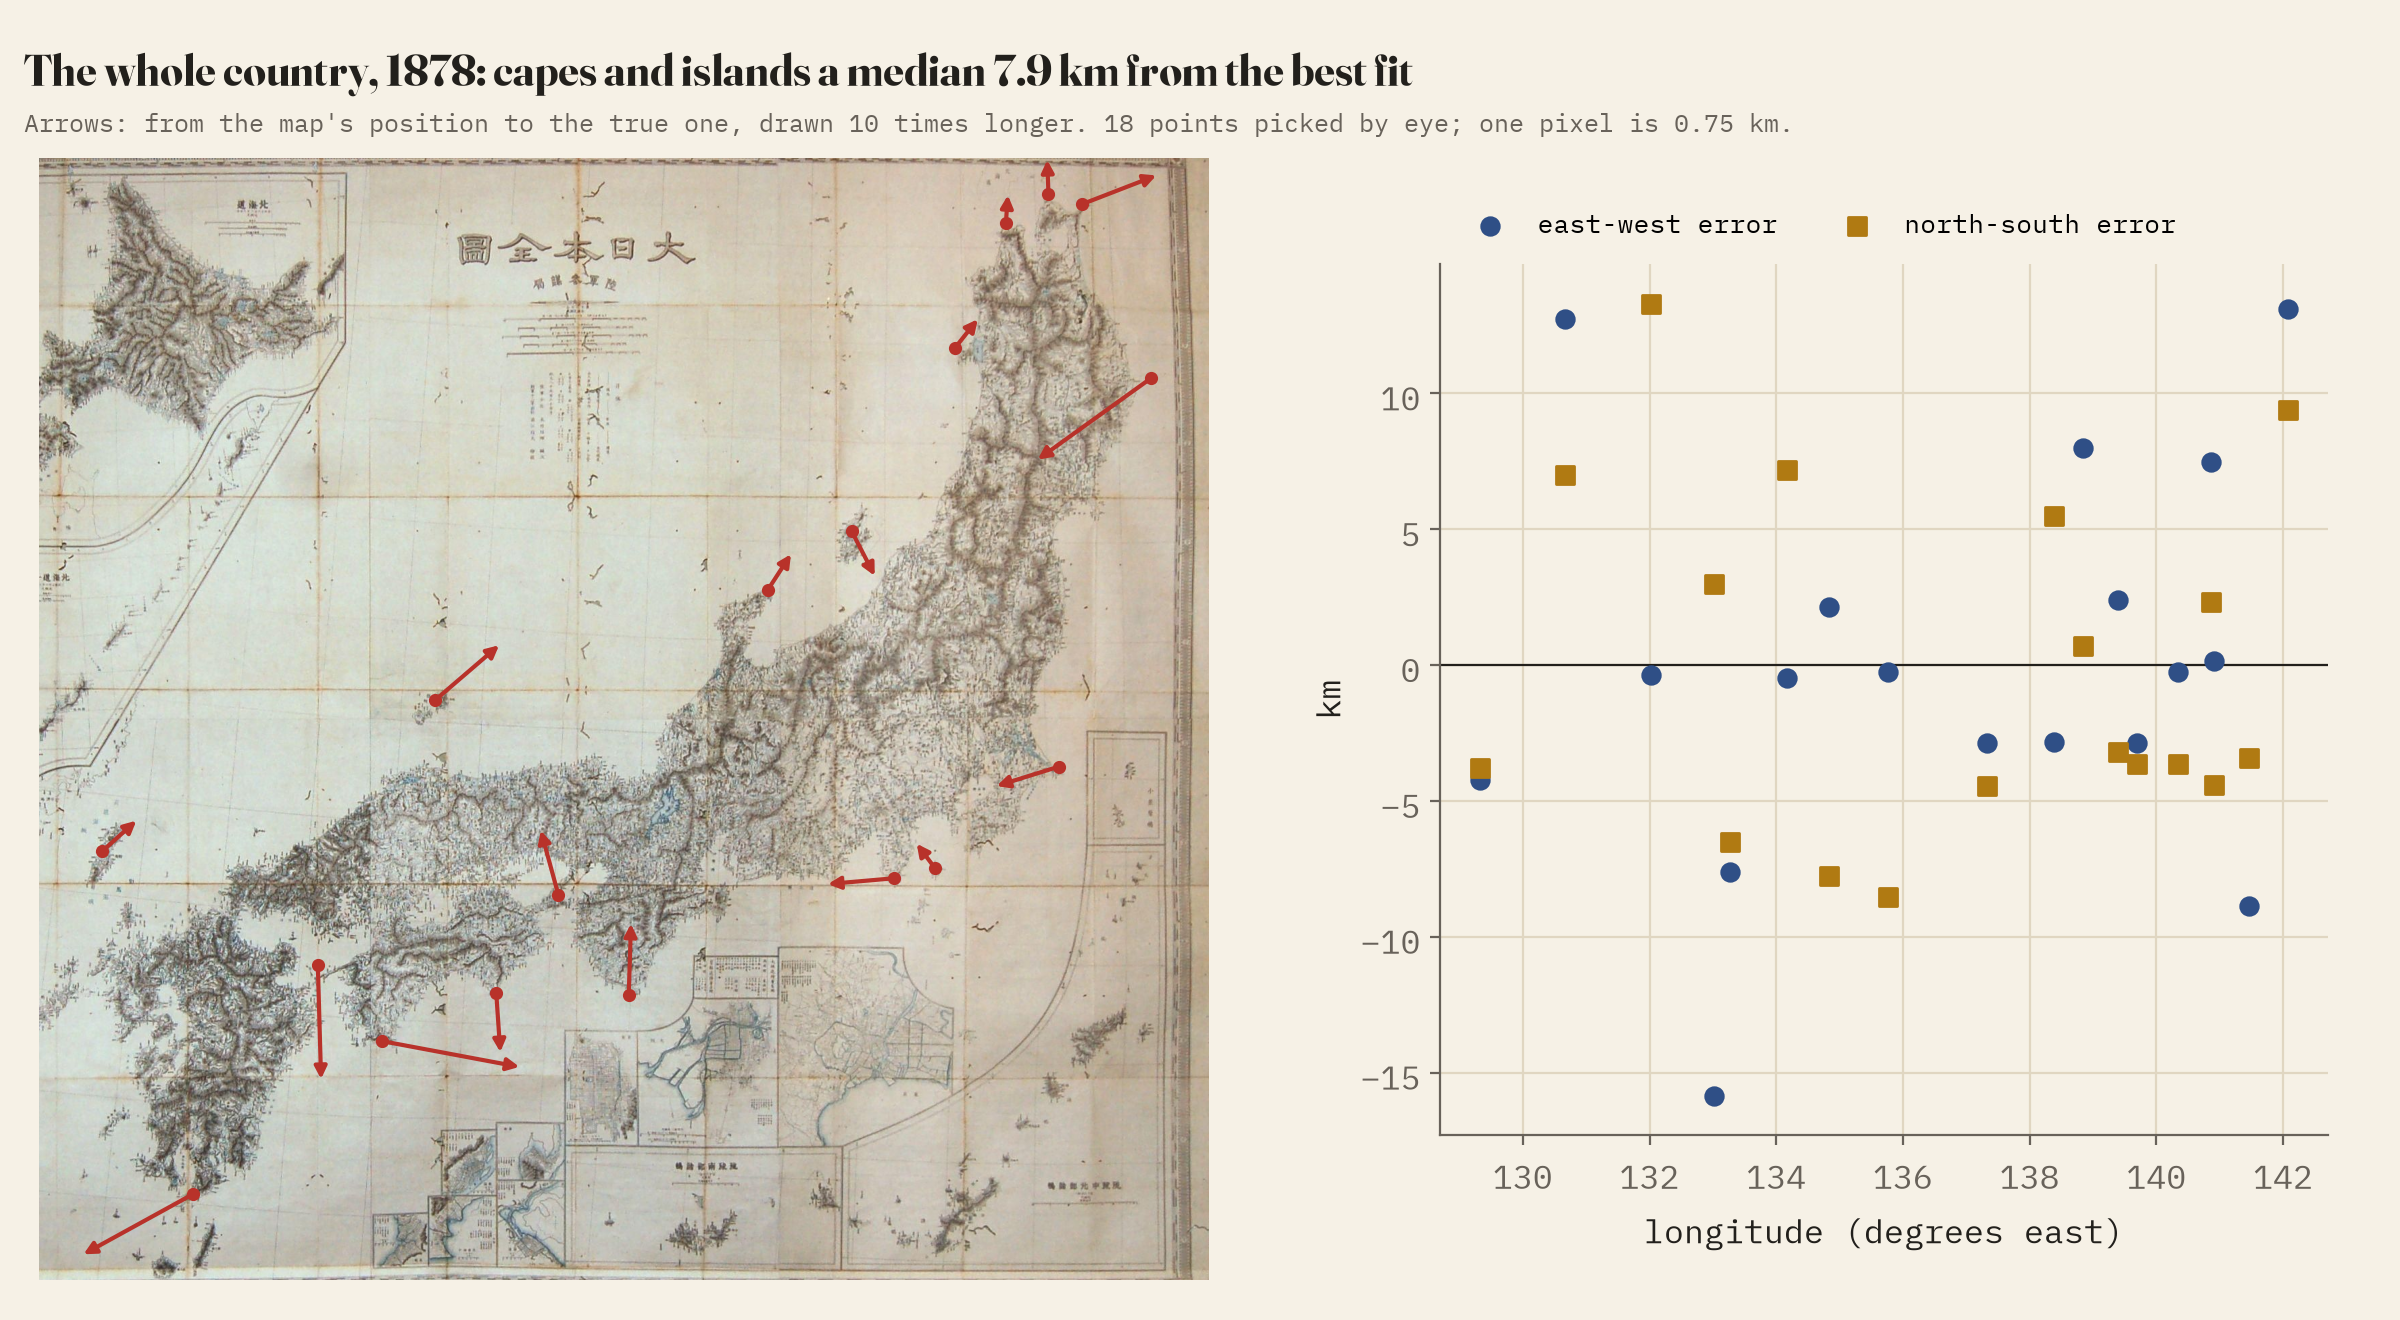
\includegraphics[width=\textwidth]{f_national.png}
\caption{Errors of 18 features on the 1878 Army General Staff map after the best similarity fit (arrows ten times longer), and their east-west and north-south parts against longitude.}\label{fig:national}\end{figure}

\begin{figure}[tbp]\centering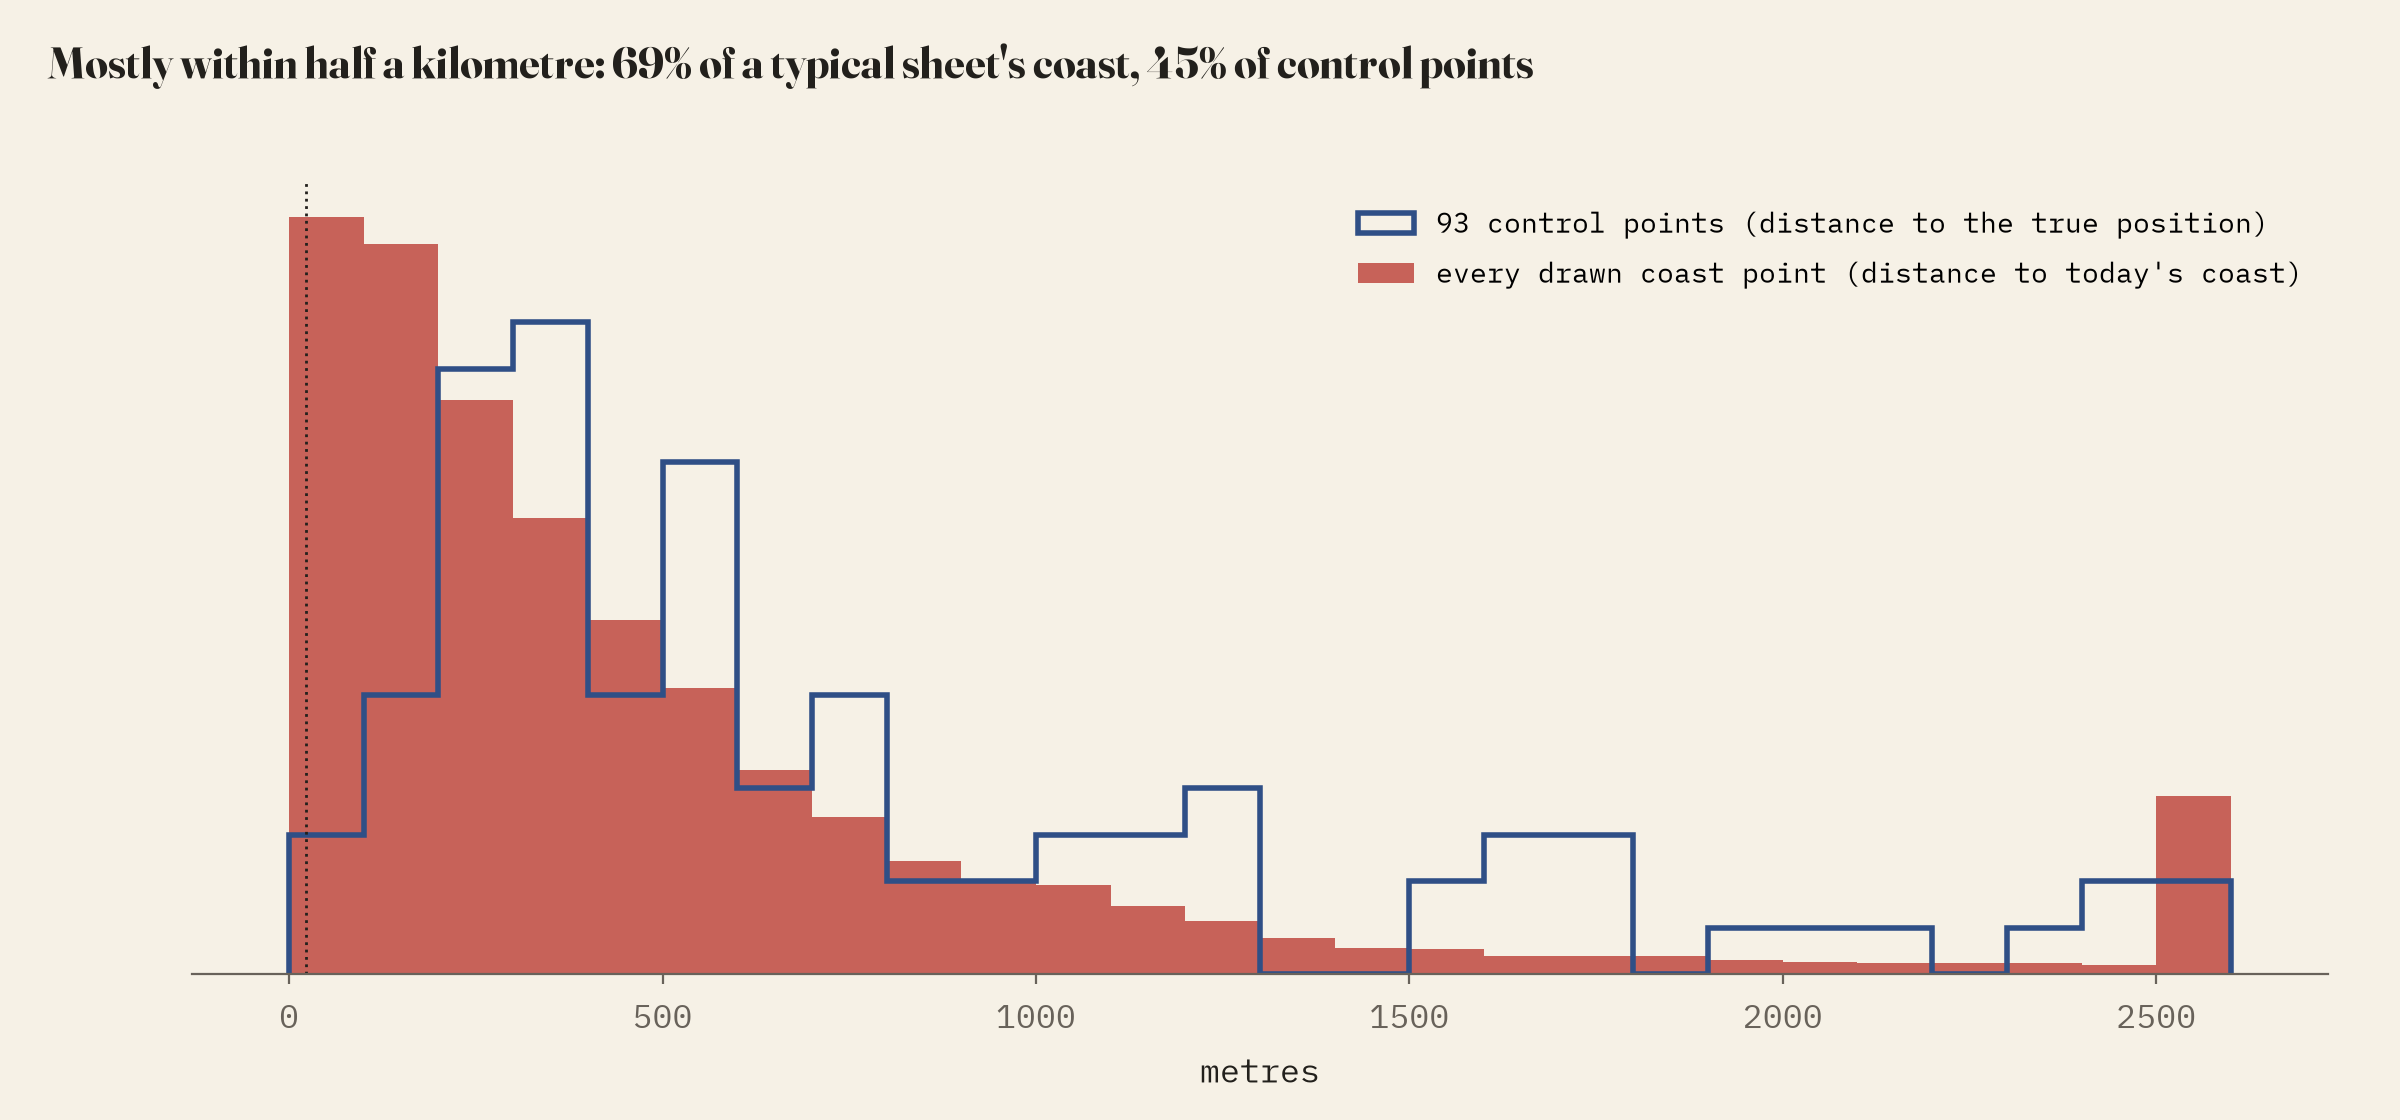
\includegraphics[width=\textwidth]{f_spread.png}
\caption{Distribution of distances from the drawn coast to the modern coast (all located sheets) and of control point errors.}\label{fig:spread}\end{figure}

\section{Limitations}
First, coverage: 40 of 214 sheets (18.7\%), all in the far north at the smaller scale, so nothing here measures the 1:36,000 sheets of Honshu, Shikoku and Kyushu. Much of the northern coast on the finished map is usually credited to Mamiya Rinzo rather than to Ino's own traverses; the results describe the map, not one surveyor. Second, the modern reference: Natural Earth's 1:10m coast is generalised for small-scale mapping and is in places several hundred metres from the true shore, so every distance here is an upper bound. Third, the sheets are a copy, photographed after folding; copying and paper distortion are included in the errors. Fourth, the scale is calibrated on one sheet and transferred by photograph size, which assumes a uniform photographic resolution. Fifth, the control points are few, and on straight coasts the rotation and along-shore position are weakly determined. Sixth, the national check rests on 18 points picked on a low-resolution photograph and on an unknown 1878 projection; the east-west stretch could come from either Ino's longitudes or the projection.

\section{Conclusion}
Within the limits of a generalised modern coastline, the northern sheets of Ino's large-scale map are accurate to a few hundred metres once each is placed: a median of 280 m along 1,494 km of coast, square to true north within about a degree or two and consistent in scale. At the national scale the 1878 map built from the survey places capes and islands within a few kilometres, and at this resolution its east-west errors are no larger than its north-south ones. A test of the main islands, and a modern coastline at survey resolution, would sharpen every figure here.

\section*{Data and code availability}
The interactive comparison is at \url{https://maps.tristanhotham.com/ino-japan/}. Data and code are at \url{https://github.com/Tristan-Hotham/ino-japan} and archived with this paper at https://doi.org/10.5281/zenodo.23882609. Derived data are released under CC BY 4.0 and code under the MIT licence. The map images are in the public domain.

\section*{AI statement}
I wrote the text, with drafting and editing assistance from Claude (Anthropic), which also helped prepare the analysis code. I reviewed and checked all text and results.

\begin{thebibliography}{9}
\bibitem[Ino(1821)]{ino} Ino Tadataka and team (1821) \textit{Dai Nihon Enkai Yochi Zenzu}, large-scale sheets, manuscript copy. Library of Congress, Geography and Map Division, item 2001620020. Photographs via Wikimedia Commons, public domain. \url{https://www.loc.gov/item/2001620020/}
\bibitem[Army General Staff Bureau(1878)]{army} Army General Staff Bureau (1878) \textit{Dai Nihon Zenzu}. Tokyo. Wikimedia Commons, public domain.
\bibitem[Natural Earth(2026)]{naturalearth} Natural Earth (2026) Admin 0 countries, 1:10m and 1:50m. Public domain. \url{https://www.naturalearthdata.com/}
\end{thebibliography}

\clearpage
\appendix
\section{The sheets}
{\footnotesize\setlength{\tabcolsep}{4pt}\begin{longtable}{rp{4.2cm}p{2.6cm}rrrrrr}\caption{The 40 sheets: area, region, length of drawn coast measured (km), median gap to the modern coast (m), share within 500 m (\%), rotation from true north (degrees, anticlockwise positive), number of control points and their median error (m).}\label{tab:sheets}\\\toprule Sheet & Area & Region & km & Gap & 500 m & Rot. & Pts & Error\\\midrule\endfirsthead\toprule Sheet & Area & Region & km & Gap & 500 m & Rot. & Pts & Error\\\midrule\endhead
1 & \multicolumn{8}{l}{\textit{not placed: a few strokes of one island only}}\\
2 & Kunashiri (middle) & Kuril islands & 42 & 446 & 57 & 1.3 & 3 & 1,032\\
3 & Kunashiri (south, Tomari) & Kuril islands & 66 & 366 & 62 & 0.2 & 13 & 986\\
4 & Iturup (Etorofu), south-west & Kuril islands & 22 & 199 & 79 & 6.1 & 3 & 371\\
5 & Rausu to the Notsuke spit & Okhotsk coast & 84 & 276 & 76 & 1.3 & 11 & 307\\
6 & Nemuro peninsula and Nemuro Bay & Nemuro and Kushiro & 76 & 285 & 70 & -1.9 & 12 & 562\\
7 & Abashiri to Shari & Okhotsk coast & 49 & 462 & 55 & 1.0 & 8 & 633\\
8 & Tokoro and Lake Saroma & Okhotsk coast & 39 & 230 & 79 & 1.5 & 2 & 275\\
9 & Sarufutsu & Okhotsk coast & 42 & 422 & 58 & -9.7 & 0 & \\
10 & Omu & Okhotsk coast & 64 & 504 & 50 & 6.2 & 0 & \\
11 & Hamatonbetsu & Okhotsk coast & 56 & 363 & 67 & -0.0 & 0 & \\
12 & west coast of southern Sakhalin & Sakhalin & 57 & 169 & 89 & -5.7 & 0 & \\
13 & Rishiri and Rebun (east coasts) & Japan Sea coast & 6 & 133 & 88 & -4.0 & 0 & \\
14 & \multicolumn{8}{l}{\textit{not placed: coast and two islands; the automatic fit failed and I could not place it with confidence}}\\
15 & Haboro & Japan Sea coast & 50 & 223 & 84 & 1.9 & 0 & \\
16 & Mashike & Japan Sea coast & 69 & 271 & 74 & 1.9 & 4 & 305\\
17 & Ishikari Bay and Otaru & Japan Sea coast & 44 & 260 & 67 & 7.3 & 1 & 2,019\\
18 & \multicolumn{8}{l}{\textit{not placed: a single small island, too little coast to place}}\\
19 & Shakotan peninsula & Japan Sea coast & 95 & 598 & 42 & 0.4 & 11 & 617\\
20 & Iwanai & Japan Sea coast & 62 & 379 & 63 & 4.1 & 8 & 565\\
21 & Akkeshi & Nemuro and Kushiro & 48 & 265 & 78 & -1.1 & 4 & 321\\
22 & Kushiro & Nemuro and Kushiro & 39 & 136 & 81 & -0.3 & 0 & \\
23 & Tokachi coast & Pacific coast & 46 & 245 & 74 & 11.6 & 0 & \\
24 & Cape Erimo & Pacific coast & 82 & 269 & 73 & 0.9 & 5 & 552\\
25 & Shizunai & Pacific coast & 61 & 651 & 40 & -8.7 & 0 & \\
26 & Hidaka-Monbetsu & Pacific coast & 33 & 108 & 95 & 1.4 & 1 & 38\\
27 & Tomakomai & Pacific coast & 60 & 566 & 44 & 0.2 & 0 & \\
28 & Muroran & Pacific coast & 32 & 436 & 58 & -1.4 & 4 & 694\\
29 & Oshamambe, Uchiura Bay & Pacific coast & 53 & 513 & 48 & -0.6 & 0 & \\
30 & Shikabe, Uchiura Bay & Pacific coast & 33 & 392 & 60 & -10.3 & 0 & \\
31 & \multicolumn{8}{l}{\textit{not placed: unfinished pencil draft of an inland route}}\\
32 & Setana & Japan Sea coast & 84 & 276 & 73 & -0.0 & 3 & 1,160\\
33 & \multicolumn{8}{l}{\textit{not placed: unfinished pencil draft}}\\
34 & \multicolumn{8}{l}{\textit{not placed: two islands sketched only}}\\
35 & \multicolumn{8}{l}{\textit{not placed: unfinished pencil draft of an inland route}}\\
36 & \multicolumn{8}{l}{\textit{not placed: unfinished pencil draft}}\\
37 & \multicolumn{8}{l}{\textit{not placed: unfinished pencil draft of inland routes}}\\
38 & \multicolumn{8}{l}{\textit{not placed: unfinished pencil draft}}\\
39 & \multicolumn{8}{l}{\textit{not placed: unfinished pencil draft, almost blank}}\\
40 & \multicolumn{8}{l}{\textit{not placed: unfinished pencil draft of inland routes}}\\
\bottomrule\end{longtable}}
\end{document}
